% !TEX root = ../main_lecture_notes.tex
\chapter{Decenralized Finance and Data Analysis}\label{chap:defi}

\section{Decentralized Finance}

Let us first list the distinctions between traditional finance (TradFi) and decentralized finance (DeFi). TradFi is often characterized by high access barriers, requiring specific criteria such as bank accounts, whereas DeFi eliminates these barriers, allowing universal participation. TradFi operates on centralized systems where banks serve as the primary record keepers, exposing them to cyber risks, whereas DeFi utilizes a decentralized ledger system, enhancing security and reducing such vulnerabilities. Moreover, TradFi is plagued by high transaction costs, including fees for account maintenance and wire transfers, and relies on intermediaries for transactions; in contrast, DeFi minimizes these costs by using smart contracts, although users must still handle gas fees. Transactions in TradFi, especially cross-border ones, can be slow, taking days to settle, while DeFi offers near-instant settlement. Furthermore, TradFi lacks transparency and can be difficult to audit, whereas DeFi provides a publicly available ledger and open-source code, ensuring greater transparency and auditability. Additionally, TradFi operations are restricted by geographical and regulatory constraints, and are often limited to business hours, while DeFi offers 24/7 global accessibility without censorship or restrictions by central authorities. TradFi's challenges in providing fractional ownership for assets like real estate and art are addressed in DeFi through the tokenization of real-world assets. Lastly, TradFi often relies on outdated IT solutions, which stifles innovation and interoperability, whereas DeFi fosters rapid innovation and enables seamless interoperability across platforms and projects. These discussion can be found for instance in the bok of \citet{Lipton2021}.

A fundamental application of DeFi are exchange platforms that allow users to trade the different kind of cryptoassets. We are going to focus on decentralized exchange in the next section.

\section{Decentralized Exchanges (DEXs) and Automated Market Makers (AMM)}

If you were to buy your first units of cryptoasset, you might turn to a centralized exchange platforms for simplicity. Centralized exchange platforms, often referred to as traditional exchanges, are operated by a central authority or company that facilitates trading between users. These exchanges offer convenience and liquidity, as well as features like advanced trading options and customer support. However, they also introduce a single point of failure and require users to trust the exchange operator with their funds and personal information, which can be vulnerable to hacks or regulatory actions. Trading on centralized exchange further also include non transparent and fluctuating transaction cost. On the other hand, decentralized exchange platforms operate on blockchain technology, allowing users to trade directly with each other without the need for an intermediary. This peer-to-peer model eliminates the need to trust a central authority and offers increased security and privacy since users retain control of their funds throughout the trading process. However, decentralized exchanges may suffer from lower liquidity and slower transaction speeds compared to centralized exchanges, and they often lack features like fiat currency support and customer service. Despite these trade-offs, decentralized exchanges are gaining popularity due to their commitment to decentralization and censorship resistance. Censorship resistance means that transactions and trading activities cannot be easily censored, blocked, or controlled by any single party, including governments or regulatory agencies.\\

\noindent \textbf{Decentralized exchanges (DEXs)} Exchange of one cryptocurrency token for another, with one token typically being more volatile or risky while the other aims to maintain stability. This pairing frequently involves a stablecoin, a type of cryptocurrency designed to minimize price volatility by pegging its value to an external reference asset, such as a fiat currency like the US dollar. Stablecoins serve as a reliable medium of exchange and store of value within the cryptocurrency ecosystem, offering traders a way to mitigate the risks associated with price fluctuations while transacting on DEXs.\\

\noindent \textbf{Stablecoins:} Two main types: fiat collateralized and crypto collateralized. 
\begin{itemize}
  \item Fiat collateralized stablecoins are backed by reserves of fiat currency, held in bank accounts or other custodial arrangements, with each stablecoin token representing a claim to a specified amount of the underlying fiat currency. Examples of fiat collateralized stablecoins include USDT (Tether), USDC (USD Coin), and BUSD (Binance USD). 
  \item Crypto collateralized stablecoins are backed by reserves of other cryptocurrencies, typically held in smart contracts or decentralized protocols, with the value of the stablecoin maintained through overcollateralization and algorithmic mechanisms, see \citet{Moin2020}. An example is provided in \cref{ex:dai}.
\end{itemize}

\begin{ex}\label{ex:dai}
One prominent example of a crypto collateralized stablecoin is DAI, which operates on the Ethereum blockchain. DAI is created and managed by the \href{https://makerdao.com/en/}{MakerDAO} protocol, a decentralized autonomous organization governed by MKR token holders. DAI is collateralized by a pool of other cryptocurrencies, primarily Ethereum (ETH), which users lock into smart contracts known as Collateralized Debt Positions (CDPs) to generate DAI tokens. The value of DAI is maintained close to one US dollar through a combination of market forces and algorithmic mechanisms, including the use of oracles to provide price feeds and the automatic adjustment of interest rates to incentivize or discourage borrowing and lending activities. By leveraging Ethereum's smart contract capabilities and a decentralized governance model, DAI offers users a transparent, trust-minimized stablecoin solution within the decentralized finance (DeFi) ecosystem.
\end{ex}

\noindent Centralized exchange use a classical order book mechanism to set the prices while DEXs use Automated Market Makers\\

\noindent \textbf{Order book-based system\footnote{\url{https://www.youtube.com/watch?v=Kl4-VJ2K8Ik}}:} buyers and sellers place orders to buy or sell assets at specific prices, creating a dynamic order book that matches buy and sell orders. This system relies on the interaction of buyers and sellers to determine the price and liquidity of assets, with prices fluctuating based on market demand and supply. This require numerous interactions with the protocol and therefore huge amounts of gas fee. The company that manage the centralized platform plays the role of market maker in a non transparent ways. It could probably be automatised within a DeFi application at the cost of writing a complex algorithm in the blockchain programming language (e.g. solidity for the Ethereum blockchain).\\

\noindent \textbf{Automated Market Makers (AMMs)} Algorithms that use liquidity pools to facilitate trading without relying on order books. AMMs determine asset prices algorithmically based on the ratio of assets in liquidity pools, providing liquidity for trades through predefined smart contracts. While order book-based systems offer more flexibility in price setting and execution, they can suffer from issues like low liquidity and price slippage, especially in volatile markets. In contrast, AMMs provide continuous liquidity and can offer lower barriers to entry for traders, but they may suffer from impermanent loss and may not always provide the best prices for large trades. Both mechanisms have their strengths and weaknesses, and their suitability depends on factors such as trading volume, market conditions, and user preferences. To learn more, the reader is referred to the following survey \citet{Xu2023}.\\

\noindent In Dexs we have two characters: The Liquidity Providers (LPs) and the exchange users.

\textbf{Liquidity Providers (LPs)} A liquidity provider is an individual or entity that deposits funds into liquidity pools on the DEX, allowing users to trade assets without needing a traditional order book or centralized intermediary.

In a decentralized exchange (DEX), liquidity providers play a crucial role in facilitating trading activities and maintaining liquidity within the exchange. A liquidity provider is an individual or entity that deposits funds into liquidity pools on the DEX, allowing users to trade assets without needing a traditional order book or centralized intermediary.

Here's how liquidity providers contribute to a DEX:

\begin{enumerate}
  \item Providing Liquidity: Liquidity providers deposit pairs of assets into liquidity pools, which are smart contracts that hold reserves of each asset. These assets are used to facilitate trades on the DEX. By contributing liquidity to the pools, providers ensure that there are sufficient funds available for users to trade with.

  \item Earning Fees: In return for providing liquidity, liquidity providers earn fees from trading activities that occur within the liquidity pools. When users execute trades on the DEX, they pay a small fee, a portion of which is distributed to liquidity providers as a reward for their contribution. This incentivizes providers to deposit funds into the liquidity pools and helps maintain liquidity on the exchange.

  \item Maintaining Price Stability: Liquidity providers help maintain price stability for assets traded on the DEX by ensuring that there are ample funds available for buying and selling. This reduces slippage—the difference between the expected price of a trade and the actual price at which the trade is executed—and improves the overall trading experience for users.

  \item Adjusting Positions: Liquidity providers may adjust their positions in the liquidity pools in response to changes in market conditions, asset prices, or trading volume. By rebalancing their holdings or adding/removing liquidity as needed, providers help optimize liquidity provision and maximize their returns.
\end{enumerate}

\textbf{Exchange User:} An exchange user refers to an individual or entity that interacts with an exchange platform to buy, sell, or trade assets. In the context of cryptocurrency exchanges, an exchange user is someone who utilizes the exchange's services to engage in trading activities involving cryptocurrencies or other digital assets.\\

\noindent The impact of trades, and liquidity provision/withdrawal on prices is governed by constant fuction market makers.\\

\noindent \textbf{Constant Function Market Makers (CFMMS:} Mathematical formula or algorithm that determines the pricing and liquidity provision mechanism within the liquidity pools. It is called "constant function" because it maintains a constant product of the quantities of two assets in the liquidity pool.\\

\noindent We focus on a prominent example of such function known as the Constant Product Market Makers Function. Consider an exchange where you can trade token $X$ for token $Y$ and conversely. The exchange starts operating as a first liquidity provider comes in and deposit $x$ of $X$ and $y$ of $Y$, therefore setting $k$ as
$$
x\cdot y = k.
$$
The liquidity provided by this LP is measured by $L = \sqrt{k} = \sqrt{x\cdot y} \text{ (geometric mean)}$.
\begin{ex}\label{ex:first_LP}
Consider a ETH$/$DAI Constant Product Market Maker. Assume that the current price for one ETH is $P=\$500$. A LP shows up and  deposits $20$ ETH plus $10,000$ DAI which sets 
$$
k = 20,000\text{ and }L = \sqrt{x\cdot y} \approx 447.
$$
\end{ex}
Assume that a trader wish to swap $X$ for $Y$ by acquiring $\text{d}y$. He then must deposit in the pool $\text{d}x$ of $X$ that solves
$$
(x+dx)(y-dy) = k\Leftrightarrow dx = \frac{x\cdot dy}{y-dy}.
$$
Trades (or swap) occur on a curve as pictured on \cref{fig:trading_curve}.
\begin{figure}[!ht]
 
 \subfloat[Initial state]{
 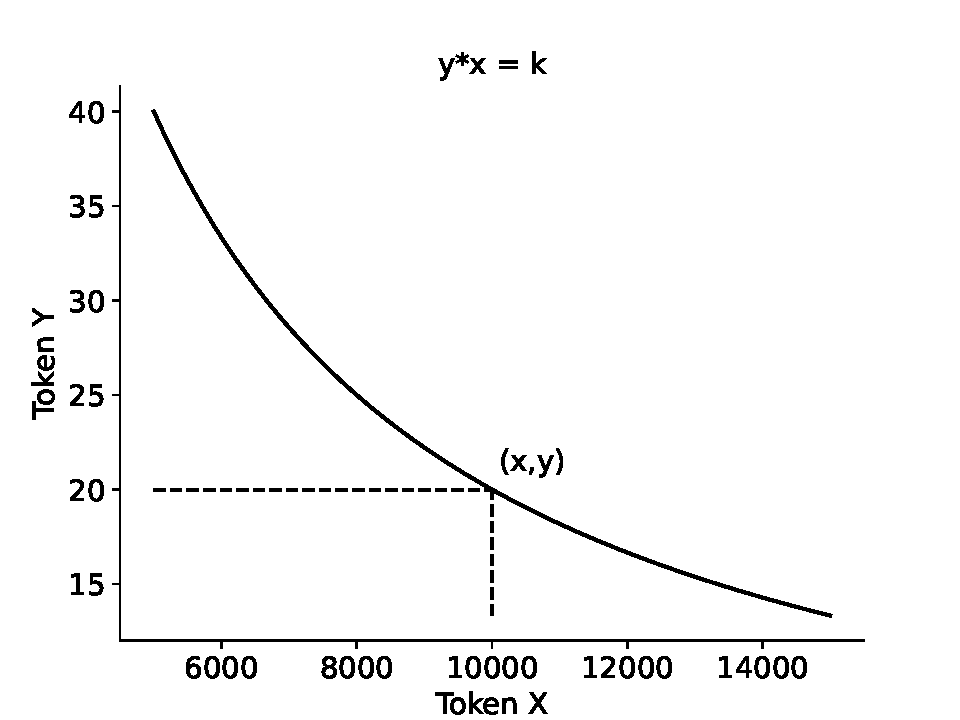
\includegraphics[width = 0.5\textwidth]{../Figures/AMM_initial.pdf}
\label{fig:initial}}
\hskip2em
\subfloat[State after the trade/swap]{
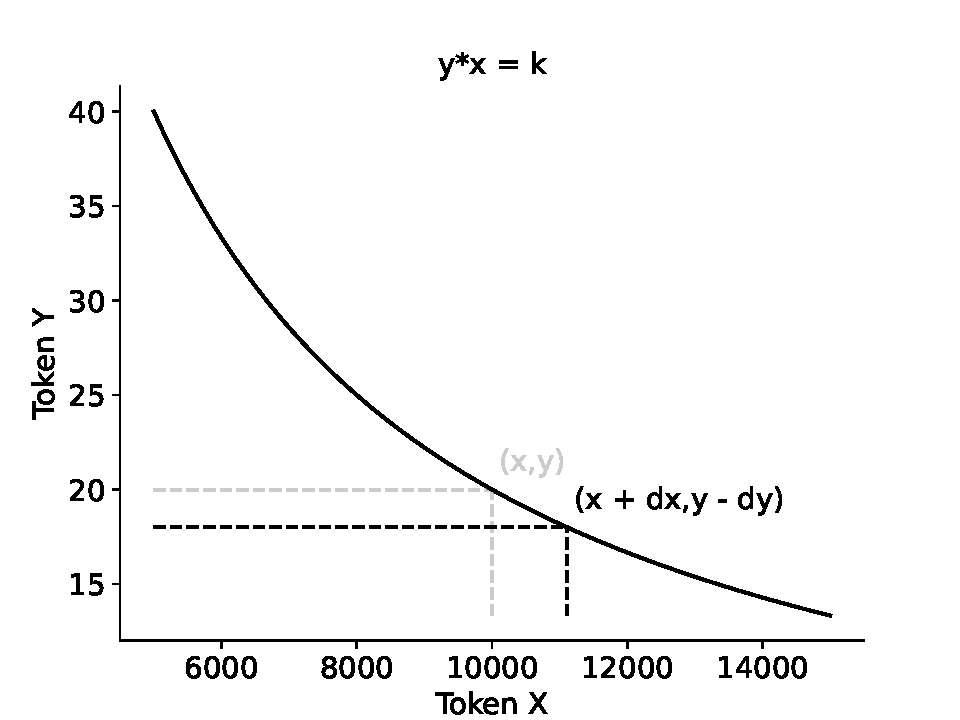
\includegraphics[width = 0.5\textwidth]{../Figures/AMM_after_swap.pdf}
\label{fig:after_swap}
}
\caption{Trade on the $x\cdot y =k$ curve.}
\label{fig:trading_curve}
\end{figure}
Usually, the protocol reward LPs by including a fee for each trade. The trader then deposits an additional $\alpha\cdot\text{d}x$ worth of fee that will be distributed to the LPs proportionnally to their Liquidity provision to the pool. Let us continue \cref{ex:first_LP} to illustrate the swap of an arbitrageur. 
\begin{ex}\label{ex:swap}
Say, an arbitrageur takes $dy=2$ ETH. She then deposits $dx = 1,111, $ and give out $0.3\cdot 1,111 = 333$ worth of fees, assuming that $\alpha = 0.3$. As a consequence, the price of ETH in the pool rises to 
      $$
      \frac{x+dx}{y-dy} = \$ 617.
      $$
\end{ex}
Another LP can provide $dx$ to the pool and therefore deposits also $dy = \frac{y}{x}dx$ so that the price does not change. The curve is bumped to a new level 
$$
k' = (x+dx)(y+dy),
$$
as shown on \cref{fig:new_k_curve}.
\begin{figure}[!ht]
\begin{center}
 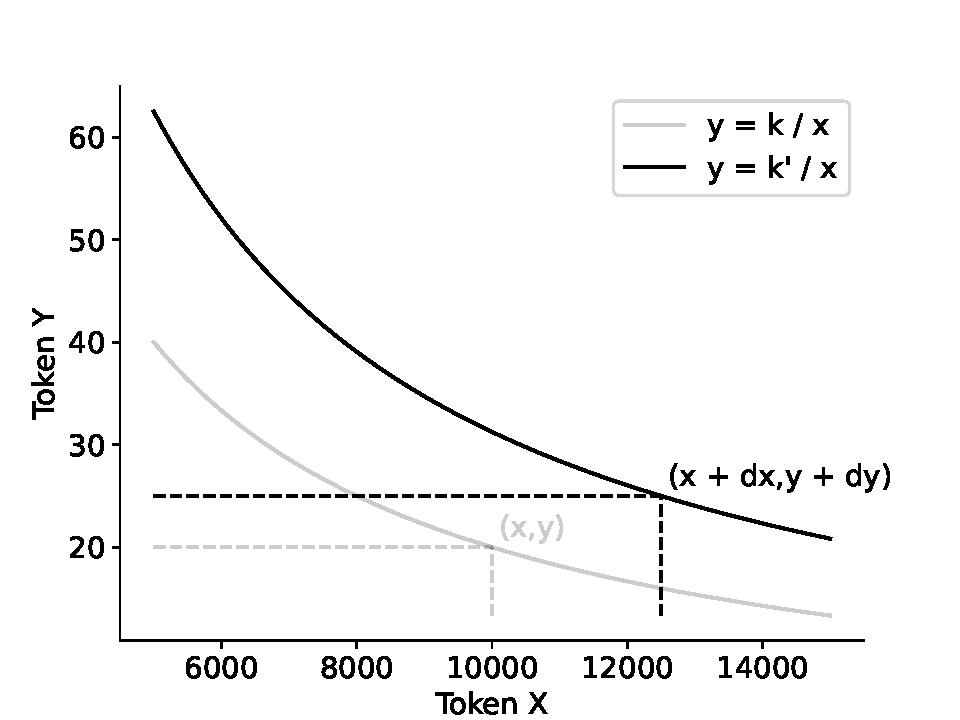
\includegraphics[width = 0.8\textwidth]{../Figures/AMM_after_drop.pdf}
\caption{Change in the curve after adding liquidity.}
\label{fig:new_k_curve}
\end{center}
\end{figure}
The overall liquidity level also rises as 
$$
L' = \sqrt{x\cdot y} + \sqrt{dx\cdot dy}.
$$
The fees are collected by both LPs accodring to the following weights 
$$
w_1=\frac{L}{L'}\text{, and }w_1=\frac{L'- L}{L'}.
$$
We resume \cref{ex:swap} with the following example
\begin{ex}\label{ex:add_liquidity}
A new LP deposits $\$5,000$ worth of tokens to the pool which splits into 
$$
dx = 2,500\text{, and }dy = 5
$$
The new levels of liquidity become 
$$
k' = 312,500\text{, and }L'\approx 559.
$$
The weights of both LPs are given by
$$
\frac{L}{L'} = 0.8\text{ and }\frac{L'-L}{L'} = 0.2.
$$
\end{ex}
AMM based DEXs commonly suffer from two things: Slippage and divergence (aka impermanent) loss. \\

\textbf{Slippage: }Slippage refers to the difference between the expected price of a trade and the actual price at which the trade is executed. When a user places a trade on an AMM-based DEX, the price of the asset may change as a result of the trade itself. This is because the constant product formula used in AMMs adjusts the price of assets based on changes in supply and demand within the liquidity pool. As a result, larger trades or trades in illiquid pools may cause significant price changes, leading to slippage. To mitigate slippage, traders can utilize strategies such as breaking up large orders into smaller ones, selecting pools with higher liquidity, or using advanced trading techniques. Additionally, ongoing improvements in AMM designs and protocols aim to minimize slippage and enhance the trading experience on decentralized exchanges. This behavior may be exploited by validating nodes of the blockachin that are aware of all the pending transaction and may front run well chosen transaction. Such an attack is described in \cref{ex:sandwich_attack} and discussed in \citet{Park2023}.

\begin{ex}[Sandwich attack]\label{ex:sandwich_attack}
The sandwich attack is a form of front-running manipulation that can occur on decentralized exchanges (DEXs) utilizing automated market makers (AMMs). In a sandwich attack, an attacker exploits the predictable price movement resulting from a large trade to profit at the expense of other traders.

Here's how the sandwich attack typically works:
\begin{enumerate}
\item Identifying the Target Transaction: The attacker monitors the blockchain for pending or recently submitted transactions that involve a large trade on a particular AMM-based DEX. Large trades can create significant price movements due to slippage, as discussed earlier.
\item Front-Running the Target Transaction: Before the target transaction is executed, the attacker quickly submits their own transactions to the DEX with the intention of exploiting the anticipated price movement caused by the large trade. The attacker strategically places buy or sell orders in such a way that they benefit from the price movement.
\item Executing Trades at Favorable Prices: As the target transaction is processed and causes the price of the asset to move, the attacker's own transactions are executed at more favorable prices due to the price impact of the large trade. This allows the attacker to buy low or sell high, effectively profiting from the price movement caused by the target transaction.
\item Exiting the Position: Once the price movement subsides, the attacker may quickly exit their position by selling or buying back the asset at a later time, potentially realizing a profit from the price difference.

\end{enumerate}
The term "sandwich attack" comes from the idea that the attacker places their own transactions on both sides of the target transaction, effectively sandwiching it between their own trades to exploit the price movement.

The sandwich attack exploits the inherent transparency and predictability of blockchain transactions, as well as the mechanics of AMMs, to profit at the expense of other traders. To mitigate the risk of sandwich attacks, traders should exercise caution when executing large trades on DEXs and consider employing strategies to minimize slippage and prevent front-running. Additionally, ongoing improvements in blockchain technology and DEX protocols aim to enhance security and protect against such attacks.
\end{ex}

\textbf{Divergence Loss:} Also known as impermanent loss, is a phenomenon that occurs when providing liquidity to an automated market maker (AMM) liquidity pool, such as those found in decentralized exchanges (DEXs). It refers to the difference in value between holding assets in the liquidity pool versus simply holding them in one's wallet.
\begin{enumerate}
\item Liquidity providers deposit pairs of assets into a liquidity pool on a DEX. For example, they may deposit equal amounts of ETH and DAI into a liquidity pool for the ETH-DAI trading pair.
\item As traders buy and sell assets on the DEX, the prices of the assets within the liquidity pool can change. These price changes can cause the ratio of the deposited assets to deviate from the initial ratio.
\item  If the price of one asset in the pool increases relative to the other, liquidity providers will have more of the asset that increased in value and less of the other asset. As a result, when they withdraw their liquidity from the pool, they will receive fewer of the appreciating asset and more of the depreciating asset compared to their initial deposit.
\item The difference in the value of the assets held in the liquidity pool compared to if they were simply held in the wallet is referred to as divergence loss or impermanent loss. 
\end{enumerate}
This loss is considered "impermanent" because it may decrease or disappear entirely if the prices of the assets revert to their initial ratio (stong assumption!!!) by the time the liquidity is withdrawn.\\

Let us consider a pool that contains token $X$ and $Y$. The price of $Y$ in the pool is given by 
$$
P = \frac{x}{y},
$$
in terms of token $X$. If the Price of $Y$ becomes $P'>P$ on another trading venue then arbitrageurs wish to find
  $$
  \underset{dy > 0}{\text{argmax }}dy\cdot P' - dx\cdot (1+\alpha) =\underset{dy}{\text{argmax }}dy\cdot P' - \frac{x\cdot dy}{y-dy}(1+\alpha). 
  $$
  Solving this optimization problem, we have 
  $$
  dy^\ast = y - \sqrt{\frac{k(1+\alpha)}{P'}}.
  $$
  The arbitrageurs profit is 
  $$
  dy^\ast\cdot P' -  dx^\ast (1+\alpha)
  $$
  which means that the LPs incur a loss of
  $$
  y\cdot P' + x - [(y-dy^\ast)\cdot P' + x + dx^\ast(1+\alpha)],
  $$
  if they withdraw. The loss is said impermanent because if the LPs do not withdraw and the price revert to the initial ratio of token in the pool then no incurred loss. Let us build on \cref{ex:add_liquidity}.
  \begin{ex}\label{ex:impermanent_loss}
  Recall that the initial price of ETH in the pool was $P = \$500$. Assume that the price in another trading venue is $P' = \$550$ and $\alpha = 0$ then 
    \begin{itemize}
      \item $dy^\ast = 0.93$
      \item The impermanent loss is then $dy^\ast\cdot P' -\frac{xdy^\ast}{y - dy^\ast} = \$23$
    \end{itemize}
    Increasing $\alpha$ then mitigate the magnitude of impermanent loss. Take $\alpha = 0.05$ tehn we have
        \begin{itemize}
      \item $dy^\ast = 0.46$
      \item The impermanent loss is then $dy^\ast\cdot P' -\frac{xdy^\ast}{y - dy^\ast} = \$5.81$.
    \end{itemize}

  \end{ex}
DEXs form a pillar of the DeFi environment but as we have seen there is room for improvement which means many avenues for future research work!












